\documentclass[twoside]{book}

% Packages required by doxygen
\usepackage{fixltx2e}
\usepackage{calc}
\usepackage{doxygen}
\usepackage{graphicx}
\usepackage[utf8]{inputenc}
\usepackage{makeidx}
\usepackage{multicol}
\usepackage{multirow}
\PassOptionsToPackage{warn}{textcomp}
\usepackage{textcomp}
\usepackage[nointegrals]{wasysym}
\usepackage[table]{xcolor}

% Font selection
\usepackage[T1]{fontenc}
\usepackage{mathptmx}
\usepackage[scaled=.90]{helvet}
\usepackage{courier}
\usepackage{amssymb}
\usepackage{sectsty}
\renewcommand{\familydefault}{\sfdefault}
\allsectionsfont{%
  \fontseries{bc}\selectfont%
  \color{darkgray}%
}
\renewcommand{\DoxyLabelFont}{%
  \fontseries{bc}\selectfont%
  \color{darkgray}%
}
\newcommand{\+}{\discretionary{\mbox{\scriptsize$\hookleftarrow$}}{}{}}

% Page & text layout
\usepackage{geometry}
\geometry{%
  a4paper,%
  top=2.5cm,%
  bottom=2.5cm,%
  left=2.5cm,%
  right=2.5cm%
}
\tolerance=750
\hfuzz=15pt
\hbadness=750
\setlength{\emergencystretch}{15pt}
\setlength{\parindent}{0cm}
\setlength{\parskip}{0.2cm}
\makeatletter
\renewcommand{\paragraph}{%
  \@startsection{paragraph}{4}{0ex}{-1.0ex}{1.0ex}{%
    \normalfont\normalsize\bfseries\SS@parafont%
  }%
}
\renewcommand{\subparagraph}{%
  \@startsection{subparagraph}{5}{0ex}{-1.0ex}{1.0ex}{%
    \normalfont\normalsize\bfseries\SS@subparafont%
  }%
}
\makeatother

% Headers & footers
\usepackage{fancyhdr}
\pagestyle{fancyplain}
\fancyhead[LE]{\fancyplain{}{\bfseries\thepage}}
\fancyhead[CE]{\fancyplain{}{}}
\fancyhead[RE]{\fancyplain{}{\bfseries\leftmark}}
\fancyhead[LO]{\fancyplain{}{\bfseries\rightmark}}
\fancyhead[CO]{\fancyplain{}{}}
\fancyhead[RO]{\fancyplain{}{\bfseries\thepage}}
\fancyfoot[LE]{\fancyplain{}{}}
\fancyfoot[CE]{\fancyplain{}{}}
\fancyfoot[RE]{\fancyplain{}{\bfseries\scriptsize Generated on Sat Dec 6 2014 02\+:54\+:19 for T\+E\+A\+C\+H\+E\+R by Doxygen }}
\fancyfoot[LO]{\fancyplain{}{\bfseries\scriptsize Generated on Sat Dec 6 2014 02\+:54\+:19 for T\+E\+A\+C\+H\+E\+R by Doxygen }}
\fancyfoot[CO]{\fancyplain{}{}}
\fancyfoot[RO]{\fancyplain{}{}}
\renewcommand{\footrulewidth}{0.4pt}
\renewcommand{\chaptermark}[1]{%
  \markboth{#1}{}%
}
\renewcommand{\sectionmark}[1]{%
  \markright{\thesection\ #1}%
}

% Indices & bibliography
\usepackage{natbib}
\usepackage[titles]{tocloft}
\setcounter{tocdepth}{3}
\setcounter{secnumdepth}{5}
\makeindex

% Hyperlinks (required, but should be loaded last)
\usepackage{ifpdf}
\ifpdf
  \usepackage[pdftex,pagebackref=true]{hyperref}
\else
  \usepackage[ps2pdf,pagebackref=true]{hyperref}
\fi
\hypersetup{%
  colorlinks=true,%
  linkcolor=blue,%
  citecolor=blue,%
  unicode%
}

% Custom commands
\newcommand{\clearemptydoublepage}{%
  \newpage{\pagestyle{empty}\cleardoublepage}%
}


%===== C O N T E N T S =====

\begin{document}

% Titlepage & ToC
\hypersetup{pageanchor=false,
             bookmarks=true,
             bookmarksnumbered=true,
             pdfencoding=unicode
            }
\pagenumbering{roman}
\begin{titlepage}
\vspace*{7cm}
\begin{center}%
{\Large T\+E\+A\+C\+H\+E\+R }\\
\vspace*{1cm}
{\large Generated by Doxygen 1.8.8}\\
\vspace*{0.5cm}
{\small Sat Dec 6 2014 02:54:19}\\
\end{center}
\end{titlepage}
\clearemptydoublepage
\tableofcontents
\clearemptydoublepage
\pagenumbering{arabic}
\hypersetup{pageanchor=true}

%--- Begin generated contents ---
\chapter{Teacher\+Basic}
\label{md__developing_programming__teacher_basics__r_e_a_d_m_e}
\hypertarget{md__developing_programming__teacher_basics__r_e_a_d_m_e}{}
A teacher program that teaches users about basics objects in C programming. 
\chapter{File Index}
\section{File List}
Here is a list of all files with brief descriptions\+:\begin{DoxyCompactList}
\item\contentsline{section}{Developing\+Programming/\+Teacher\+Basics/\hyperlink{_teacher_basics_8c}{Teacher\+Basics.\+c} }{\pageref{_teacher_basics_8c}}{}
\end{DoxyCompactList}

\chapter{File Documentation}
\section{Developing\+Programming/\+Developing\+Computer\+Programming/\+R\+E\+A\+D\+M\+E.md File Reference}
\label{_r_e_a_d_m_e_8md}\index{Developing\+Programming/\+Developing\+Computer\+Programming/\+R\+E\+A\+D\+M\+E.\+md@{Developing\+Programming/\+Developing\+Computer\+Programming/\+R\+E\+A\+D\+M\+E.\+md}}

\hypertarget{_teacher_basics_8c}{\section{Developing\+Programming/\+Teacher\+Basics/\+Teacher\+Basics.c File Reference}
\label{_teacher_basics_8c}\index{Developing\+Programming/\+Teacher\+Basics/\+Teacher\+Basics.\+c@{Developing\+Programming/\+Teacher\+Basics/\+Teacher\+Basics.\+c}}
}
{\ttfamily \#include $<$stdio.\+h$>$}\\*
{\ttfamily \#include $<$string.\+h$>$}\\*
Include dependency graph for Teacher\+Basics.\+c\+:\nopagebreak
\begin{figure}[H]
\begin{center}
\leavevmode
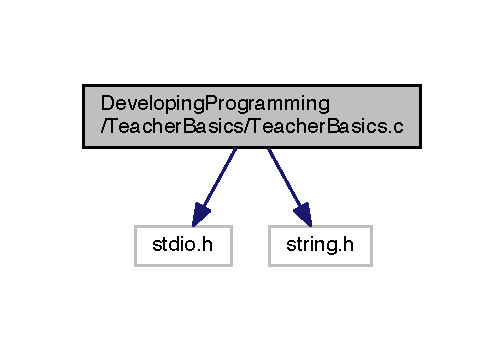
\includegraphics[width=242pt]{_teacher_basics_8c__incl}
\end{center}
\end{figure}
\subsection*{Functions}
\begin{DoxyCompactItemize}
\item 
void \hyperlink{_teacher_basics_8c_ad0bea7ca09a6fd8663f0c0f7ac219c20}{Data\+Types} ()
\item 
void \hyperlink{_teacher_basics_8c_a6ef0cf8d139194a7cc30e0c64e09b14e}{Modifiers} ()
\item 
int \hyperlink{_teacher_basics_8c_ae66f6b31b5ad750f1fe042a706a4e3d4}{main} ()
\end{DoxyCompactItemize}
\subsection*{Variables}
\begin{DoxyCompactItemize}
\item 
const int \hyperlink{_teacher_basics_8c_af7dbda7167e22cb3417c16f78061ad80}{M\+A\+X} =2
\end{DoxyCompactItemize}


\subsection{Function Documentation}
\hypertarget{_teacher_basics_8c_ad0bea7ca09a6fd8663f0c0f7ac219c20}{\index{Teacher\+Basics.\+c@{Teacher\+Basics.\+c}!Data\+Types@{Data\+Types}}
\index{Data\+Types@{Data\+Types}!Teacher\+Basics.\+c@{Teacher\+Basics.\+c}}
\subsubsection[{Data\+Types}]{\setlength{\rightskip}{0pt plus 5cm}void Data\+Types (
\begin{DoxyParamCaption}
{}
\end{DoxyParamCaption}
)}}\label{_teacher_basics_8c_ad0bea7ca09a6fd8663f0c0f7ac219c20}




Original Author\+: Nishant Jain

File Creation Date\+: 22 November 2014

Description\+: A program that teaches the user about different data types and modifiers



 Module Name\+: Data\+Types

Original Author\+: Nishant Jain

Module Creation Date\+: November 23, 2014

Description\+: This function teaches user about different data types

Required Files/\+Databases\+: None

Non System Routines Called\+: None

Return Value\+: None

O\+S Specific Assumptions\+: None

Local Variables\+: ch char-\/array Used to take input for user's choice i int Used in do-\/while loop to reapeat loop on incorrect input 

Definition at line 107 of file Teacher\+Basics.\+c.



Referenced by main().


\begin{DoxyCode}
108 \{
109   \textcolor{comment}{//local variable, array}
110   \textcolor{keywordtype}{char} ch[10];
111   \textcolor{keywordtype}{int} i;
112 
113   printf(\textcolor{stringliteral}{"\(\backslash\)nThere are four basic data types: char-character, "}
114   \textcolor{stringliteral}{"int-integer, float, and double. \(\backslash\)n"});
115   
116   \textcolor{keywordflow}{do}
117   \{
118     printf(\textcolor{stringliteral}{"Which data type do you want to learn about? \(\backslash\)n"});
119     scanf(\textcolor{stringliteral}{" %s"}, ch);
120     i=0;
121     
122     \textcolor{comment}{/*}
123 \textcolor{comment}{    * Conditions for user's choice of subject. }
124 \textcolor{comment}{    * Following can be interpreted as a database of req. info. on subject}
125 \textcolor{comment}{    * Using <strcmp> to compare strings}
126 \textcolor{comment}{    */}
127     \textcolor{keywordflow}{if}(strcmp(ch,\textcolor{stringliteral}{"char"})==0)
128     \{
129       printf(\textcolor{stringliteral}{"char is a data type used to store a single "}
130       \textcolor{stringliteral}{"character such as a number, text or special characters. \(\backslash\)n"}
131       \textcolor{stringliteral}{"Storage size: %lu bytes \(\backslash\)nValue "}
132       \textcolor{stringliteral}{"Range:-128 to 127 or 0 to 255 \(\backslash\)n"}, \textcolor{keyword}{sizeof}(\textcolor{keywordtype}{char}));
133     \}
134     
135     \textcolor{keywordflow}{else} \textcolor{keywordflow}{if}(strcmp(ch,\textcolor{stringliteral}{"int"})==0)
136     \{  
137       printf(\textcolor{stringliteral}{"int is a data type used to store numerical data. \(\backslash\)n"}
138       \textcolor{stringliteral}{"Storage size: %lu bytes  \(\backslash\)nValue "}
139       \textcolor{stringliteral}{"Range:-32,768 to 32,767  \(\backslash\)n"}, \textcolor{keyword}{sizeof}(\textcolor{keywordtype}{int}));
140     \}
141 
142     \textcolor{keywordflow}{else} \textcolor{keywordflow}{if}(strcmp(ch,\textcolor{stringliteral}{"float"})==0)
143     \{
144       printf(\textcolor{stringliteral}{"float is a data type used "}
145       \textcolor{stringliteral}{"to store decimal numbers up to 6 decimal places. \(\backslash\)n"} 
146       \textcolor{stringliteral}{"Storage size: %lu bytes  \(\backslash\)nValue "}
147       \textcolor{stringliteral}{"Range:1.2E-38 to 3.4E+38 \(\backslash\)n"}, \textcolor{keyword}{sizeof}(\textcolor{keywordtype}{float}));
148     \}
149 
150     \textcolor{keywordflow}{else} \textcolor{keywordflow}{if}(strcmp(ch,\textcolor{stringliteral}{"double"})==0)
151     \{
152       printf(\textcolor{stringliteral}{"double is a data type used "}
153       \textcolor{stringliteral}{"to store decimal numbers to up to 15 decimal places . \(\backslash\)n"}
154       \textcolor{stringliteral}{"Storage size: %lu bytes \(\backslash\)nValue "}
155       \textcolor{stringliteral}{"Range:2.3E-308 to 1.7E+308 \(\backslash\)n"}, \textcolor{keyword}{sizeof}(\textcolor{keywordtype}{double}));
156     \}
157 
158     \textcolor{keywordflow}{else}
159     \{ 
160       \textcolor{comment}{//Repeating the input if an error}
161       printf(\textcolor{stringliteral}{"Input either 'char', 'int', 'float' or 'double'. \(\backslash\)n"});
162       i=1;
163     \}  
164   \}\textcolor{keywordflow}{while}(i==1);
165 \}
\end{DoxyCode}


Here is the caller graph for this function\+:\nopagebreak
\begin{figure}[H]
\begin{center}
\leavevmode
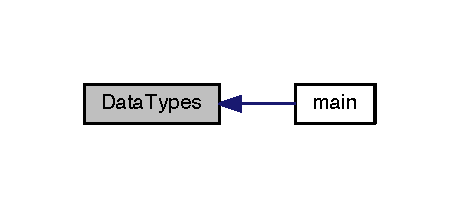
\includegraphics[width=220pt]{_teacher_basics_8c_ad0bea7ca09a6fd8663f0c0f7ac219c20_icgraph}
\end{center}
\end{figure}


\hypertarget{_teacher_basics_8c_ae66f6b31b5ad750f1fe042a706a4e3d4}{\index{Teacher\+Basics.\+c@{Teacher\+Basics.\+c}!main@{main}}
\index{main@{main}!Teacher\+Basics.\+c@{Teacher\+Basics.\+c}}
\subsubsection[{main}]{\setlength{\rightskip}{0pt plus 5cm}int main (
\begin{DoxyParamCaption}
{}
\end{DoxyParamCaption}
)}}\label{_teacher_basics_8c_ae66f6b31b5ad750f1fe042a706a4e3d4}


 Module Name\+: main

Original Author\+: Nishant

Module Creation Date\+: November 22, 2014

Description\+: Calls \hyperlink{_teacher_basics_8c_ad0bea7ca09a6fd8663f0c0f7ac219c20}{Data\+Types()} and Modifiers acc. to user's choice

Required Files/\+Databases\+: None

Non System Routines Called\+: None

Return Value\+: Type Description int return(0)

O\+S Specific Assumptions\+: None

Local Variables\+: Name Type Description check char To see if user wants to continue ch int User's choice of operation cont char To ask if user wants to continue or not 

Definition at line 49 of file Teacher\+Basics.\+c.



References Data\+Types(), and Modifiers().


\begin{DoxyCode}
50 \{
51  \textcolor{keywordtype}{int} ch;
52  \textcolor{keywordtype}{char} cont;
53  
54  \textcolor{keywordflow}{do}
55  \{
56    printf(\textcolor{stringliteral}{"Hello there! I am your teacher for the day. \(\backslash\)n"});
57    printf(\textcolor{stringliteral}{"What do you want to learn? \(\backslash\)n 1)Data Types \(\backslash\)n 2)Modifiers"});
58    scanf(\textcolor{stringliteral}{" %d"}, &ch);
59 
60    \textcolor{keywordflow}{if}(ch==1)
61    \{
62      \hyperlink{_teacher_basics_8c_ad0bea7ca09a6fd8663f0c0f7ac219c20}{DataTypes}();
63    \}
64    
65    \textcolor{keywordflow}{else} \textcolor{keywordflow}{if}(ch==2)
66    \{
67     \hyperlink{_teacher_basics_8c_a6ef0cf8d139194a7cc30e0c64e09b14e}{Modifiers}();
68    \}
69  
70    \textcolor{keywordflow}{else} printf(\textcolor{stringliteral}{"Select a valid option."});
71    \textcolor{comment}{//Asking user to continue}
72    printf(\textcolor{stringliteral}{"Continue (Y/N)? \(\backslash\)n"});
73    scanf(\textcolor{stringliteral}{" %c"}, &cont);
74    
75  \}\textcolor{keywordflow}{while} (cont==\textcolor{charliteral}{'Y'} || cont==\textcolor{charliteral}{'y'});
76  
77  
78  \textcolor{keywordflow}{return} (0);
79 \}  
\end{DoxyCode}


Here is the call graph for this function\+:\nopagebreak
\begin{figure}[H]
\begin{center}
\leavevmode
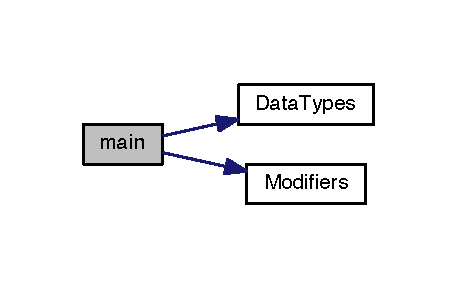
\includegraphics[width=220pt]{_teacher_basics_8c_ae66f6b31b5ad750f1fe042a706a4e3d4_cgraph}
\end{center}
\end{figure}


\hypertarget{_teacher_basics_8c_a6ef0cf8d139194a7cc30e0c64e09b14e}{\index{Teacher\+Basics.\+c@{Teacher\+Basics.\+c}!Modifiers@{Modifiers}}
\index{Modifiers@{Modifiers}!Teacher\+Basics.\+c@{Teacher\+Basics.\+c}}
\subsubsection[{Modifiers}]{\setlength{\rightskip}{0pt plus 5cm}void Modifiers (
\begin{DoxyParamCaption}
{}
\end{DoxyParamCaption}
)}}\label{_teacher_basics_8c_a6ef0cf8d139194a7cc30e0c64e09b14e}


 Module Name\+: Modifiers

Original Author\+: Nishant Jain

Module Creation Date\+: November 23, 2014

Description\+: This function teaches user about different Modifiers

Required Files/\+Databases\+: None

Non System Routines Called\+: None

Return Value\+: None

O\+S Specific Assumptions\+: None

Local Variables\+: ch char-\/array Used to take input for user's choice i int Used in do-\/while loop to reapeat loop on incorrect input 

Definition at line 194 of file Teacher\+Basics.\+c.



Referenced by main().


\begin{DoxyCode}
195 \{
196   \textcolor{comment}{//local variable, string}
197   \textcolor{keywordtype}{char} ch[10];
198   \textcolor{keywordtype}{int} i;
199 
200   printf(\textcolor{stringliteral}{"\(\backslash\)nThere are five basic modifiers: signed, unsigned, short,"}
201   \textcolor{stringliteral}{" long and const-constant. \(\backslash\)n"});
202   
203   \textcolor{keywordflow}{do}
204   \{
205     i=0;
206     printf(\textcolor{stringliteral}{"Which modifier do you want to learn about? \(\backslash\)n"});
207     scanf(\textcolor{stringliteral}{" %s"}, ch);
208     
209     \textcolor{comment}{/*}
210 \textcolor{comment}{    * Conditions for user's choice of subject. }
211 \textcolor{comment}{    * Following can be interpreted as a database of req. info. on subject}
212 \textcolor{comment}{    */}
213     \textcolor{keywordflow}{if}(strcmp(ch,\textcolor{stringliteral}{"signed"})==0)
214     \{
215       printf(\textcolor{stringliteral}{"All data types are “signed” by default. Signed"}
216       \textcolor{stringliteral}{" Data Modifier implies that the data type variable can"}
217       \textcolor{stringliteral}{" store positive values as well as negative values."}
218       \textcolor{stringliteral}{" \(\backslash\)nFor example: signed int temperature; \(\backslash\)n"});
219 
220       printf(\textcolor{stringliteral}{"Size of signed int is %lu bytes\(\backslash\)n"}, \textcolor{keyword}{sizeof}(\textcolor{keywordtype}{signed} \textcolor{keywordtype}{int}));
221       printf(\textcolor{stringliteral}{"Size of signed char is %lu bytes\(\backslash\)n"}, \textcolor{keyword}{sizeof}(\textcolor{keywordtype}{signed} \textcolor{keywordtype}{char}));
222 
223     \}
224 
225     \textcolor{keywordflow}{else} \textcolor{keywordflow}{if}(strcmp(ch,\textcolor{stringliteral}{"unsigned"})==0)
226     \{
227       printf(\textcolor{stringliteral}{"If we need to change the data type so that it"}
228       \textcolor{stringliteral}{" can only store only store positive values,"}
229       \textcolor{stringliteral}{" “unsigned” data modifier is used."}
230       \textcolor{stringliteral}{" \(\backslash\)nFor example: unsigned int salary; \(\backslash\)n"});
231 
232       printf(\textcolor{stringliteral}{"Size of unsigned int is %lu bytes\(\backslash\)n"}, \textcolor{keyword}{sizeof}(\textcolor{keywordtype}{unsigned} \textcolor{keywordtype}{int}));
233       printf(\textcolor{stringliteral}{"Size of unsigned short is %lu bytes\(\backslash\)n"}, \textcolor{keyword}{sizeof}(\textcolor{keywordtype}{unsigned} \textcolor{keywordtype}{short}));
234       printf(\textcolor{stringliteral}{"Size of unsigned long is %lu bytes\(\backslash\)n"}, \textcolor{keyword}{sizeof}(\textcolor{keywordtype}{unsigned} \textcolor{keywordtype}{long}));
235     \} 
236 
237     \textcolor{keywordflow}{else} \textcolor{keywordflow}{if}(strcmp(ch,\textcolor{stringliteral}{"short"})==0)
238     \{
239       printf(\textcolor{stringliteral}{"A “short” type modifier does"}
240       \textcolor{stringliteral}{" just the opposite of “long”. If one is not expecting"}
241       \textcolor{stringliteral}{" to see high range values in a program and the values"}
242       \textcolor{stringliteral}{" are both positive & negative."}
243       \textcolor{stringliteral}{" \(\backslash\)nFor example: short int age; \(\backslash\)n"});
244     \}
245 
246     \textcolor{keywordflow}{else} \textcolor{keywordflow}{if}(strcmp(ch,\textcolor{stringliteral}{"long"})==0)
247     \{ 
248       printf(\textcolor{stringliteral}{"Sometimes while coding a program,"}
249       \textcolor{stringliteral}{" we need to increase the Storage Capacity of a variable"}
250       \textcolor{stringliteral}{" so that it can store values higher than its maximum limit,"}
251       \textcolor{stringliteral}{" which is there as default. In such situations or programs,"}
252       \textcolor{stringliteral}{" we need to make use of the “long” data type qualifier."}
253       \textcolor{stringliteral}{" “long” type modifier doubles the “length” of the data"}
254       \textcolor{stringliteral}{" type when used along with it."}
255       \textcolor{stringliteral}{" \(\backslash\)nFor example: long int turnover; \(\backslash\)n"});
256 
257       printf(\textcolor{stringliteral}{"Size of long double is %lu bytes\(\backslash\)n"}, \textcolor{keyword}{sizeof}(\textcolor{keywordtype}{long} \textcolor{keywordtype}{double}));
258     \}
259 
260     \textcolor{keywordflow}{else} \textcolor{keywordflow}{if}(strcmp(ch,\textcolor{stringliteral}{"const"})==0)
261     \{
262       printf(\textcolor{stringliteral}{"const sets the value of variable as"}
263       \textcolor{stringliteral}{" constants. If the program tries to change the value of a"}
264       \textcolor{stringliteral}{" constant variable, it displays an error. \(\backslash\)nFor example:"}
265       \textcolor{stringliteral}{" const int MAX=2; (Has been declared in the beginning.) \(\backslash\)n"});
266     \}
267 
268     \textcolor{keywordflow}{else} 
269     \{ 
270       \textcolor{comment}{//Repeating the input if an error }
271       printf(\textcolor{stringliteral}{"Input either 'signed', 'unsigned', 'short',"}
272       \textcolor{stringliteral}{" 'const' or 'long'. \(\backslash\)n"});
273       i=1;
274     \}
275   \}\textcolor{keywordflow}{while}(i==1);
276 \}\end{DoxyCode}


Here is the caller graph for this function\+:\nopagebreak
\begin{figure}[H]
\begin{center}
\leavevmode
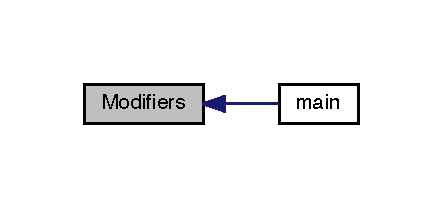
\includegraphics[width=212pt]{_teacher_basics_8c_a6ef0cf8d139194a7cc30e0c64e09b14e_icgraph}
\end{center}
\end{figure}




\subsection{Variable Documentation}
\hypertarget{_teacher_basics_8c_af7dbda7167e22cb3417c16f78061ad80}{\index{Teacher\+Basics.\+c@{Teacher\+Basics.\+c}!M\+A\+X@{M\+A\+X}}
\index{M\+A\+X@{M\+A\+X}!Teacher\+Basics.\+c@{Teacher\+Basics.\+c}}
\subsubsection[{M\+A\+X}]{\setlength{\rightskip}{0pt plus 5cm}const int M\+A\+X =2}}\label{_teacher_basics_8c_af7dbda7167e22cb3417c16f78061ad80}


Definition at line 18 of file Teacher\+Basics.\+c.


%--- End generated contents ---

% Index
\newpage
\phantomsection
\addcontentsline{toc}{chapter}{Index}
\printindex

\end{document}
